\documentclass[
    load-dhbw-templates,
    load-preamble = true,
    auto-intro-pages = all,
    add-tocs-to-toc,
    debug = true,
    language = english,
    mainlanguage = ngerman,
    add-bibliography,
    bib-file = dhbw-source.bib,
    biblatex/style = alphabetic, 
]{iodhbwm}

\usepackage[T1]{fontenc}
\usepackage[printonlyused,withpage]{acronym}
\usepackage{nameref}
\usepackage{verbatim}
\usepackage{graphicx}
\usepackage{outlines}
\usepackage{pifont}
\usepackage{multirow}
\usepackage{enumitem}
\usepackage{float}


%TODO
\dhbwsetup{%
	intro/append custom content = {\listofappendices},
	dhbw location			= Mannheim,
	abstract				= abstract.tex,
    author                  = Belana Roman \& Noah Wiederhold,
    date					= [Datum],
    submission date			= [Abgabe Datum],
    thesis type             = SA,
    thesis title            = [Thema],
    student id              = <Matrikelnummer>,
    institute               = Deutsches Zentrum für Luft- und Raumfahrt,
   	institute section		= Institut für Flugsystemtechnik - Flugdynamik und Simulation,
   	institute logo			= ../Fotos/Standard/Logo-DLR,
    course/id               = TINF20IT1,
    course/name				= Informationstechnik,
    supervisor              = <Name des Betreuers>,
    processing period       = {24.12.2020 - 02.04.2021,28.06.2021- 30.09.2021},
    location                = Mannheim
    
}

% Rename appendix name
\renewcommand{\listappendixname}{Anhangsverzeichnis}

%\ExecuteBibliographyOptions{hyperref=true}
\begin{document}
    

$
%	Abkürzungen:
%	\ac{Bezeichner}
%
%	Verweise deklarieren:
%	\label{sec:Bezeichner}
% 	\label{fig:Bezeichner}
%
%	Verweise setzen:
%	(siehe \ref{sec:Bez} \nameref{sec:Bez} auf Seite \pageref{sec:Bez})
%
%	Grafiken einfügen:
%	\begin{figure}[!hbpt]
%	\centering
%	\includegraphics[scale=0.7]{pictures/schema/osg_mit_opengl_ebenen.PNG}
%	\caption[OSG Ebenen]{Ebenen einer Anwendung mit OSG Einbindung}
%	\label{fig:OSG_Ebenen} 
%	\end{figure}
%	
%	Text hervorheben:
%	\texttt{Text}
%
%	Text zentrieren:
%	\begin{center}
%	Text
%	\end{center}
%
%	Pfeil nach rechts:
%	\\rightarrow
%
%	Anführungszeichen:
%	"'Text"'
%
%	Erzwinge Ausgabe von Grafiken, etc. an bestimmtem Punkt:
%	\clearpage
%
%	Erzwinge neue Seite:
%	\newpage
%
%	Aufzählung:
%	\begin{center}
%	\begin{itemize}
%	\item Text
%	\end{itemize}
%	\end{center}
$   
$    
%	\chapter{Hauptebene}
%
%	\section{Ebene 1}
%
%	\subsection{Ebene 2}
%
%	\subsubsection{Ebene 3}
%
%	\subsubsection*{Ebene 3 ohne Aufzählung}
$
\chapter{Einleitung}
    \section{Motivation}
    Innerhalb eines dualen Studiums ist das Wechseln der Standorte zwischen Theorie- und Praxisphasen ein zentraler Bestandteil des Alltages. Der Wechsel findet dabei meist alle 3 Monate statt, und hat je nach Entfernung der beiden Standorte häufig auch einen Wechsel des Wohnortes für diese Zeit zur Folge. Bei der Haltung beziehungsweise Zucht von Pflanzen stehen wir Studenten daher vor einigen Herausforderungen.
    Entweder die Pflanzen müssen alle drei Monaten zum nächsten Standort transportiert werden, oder es müssen stets neue Pflanzen gezüchtet beziehungsweise gekauft werden. Um solche Probleme anzugehen, gibt es auf dem Markt einige vollautomatische Smart-Garden-Systeme, die den Anbau von Pflanzen in jeder Wohnung ermöglichen sollen und die Pflanzen dabei selbstständig mit Wasser, Licht und Nährstoffen versorgen. Innerhalb solcher Systeme finden allerdings nur wenige Pflanzen Platz und je umfangreicher ein solches System sein soll, desto schneller steigt auch der Preis dafür.

    Ziel dieser Arbeit ist daher die Entwicklung einer eigenständigen digitale Überwachung und automatisierten Pflege von Pflanzen im eigenen Zuhause, um eine Möglichkeit zur Erhaltung von Pflanzen über längere Abwesenheiten hinweg zu schaffen.

    %TODO Detaillierter Beschreiben wie? Mit Webserver etc.?
    \section{Zielsetzung}
    Innerhalb des zu entwickelnden Systems sollen verschiedenen Parametern bezüglich des Pflanzenwachstums, darunter die Bodenfeuchte der Erde sowie die Temperatur im Raum überwacht und schließlich für den Anwender geeignet dargestellt werden, sodass eine Überwachung der Pflanzen auch aus der Ferne möglich wird.  
    Auf die gemessenen Parameter soll das Überwachungssystem darüber hinaus auch entsprechend mit automatischen Systemen, wie einem automatischen Bewässerungssystem, reagieren.

    Das so entwickelte digitale Gartensystem lässt sich schließlich individuell anpassen und beliebig um weitere Parameter oder weitere Pflanzen erweitern.

\chapter{Strukturierte Aufgabenstellung} 
    (verifizierbar, validierbar)

    Aufgabe 1 
    Darstellung der theoretischen Grundlagen
    1.1 arduinou
    1.2 arduino uno
    1.3 Sensoren
    1.3.1 Feuchtigkeitssensore
    ...
    Aufgabe 2
    Entwicklung eines Konzepts
    2.1 Zusammenhang Module
    Schnittstellen
    Wie sollen Daten ausgetauscht werden
    2.2 Modul Arduino
    2.3 Modul Web...
    Aufgabe 3
    Implementierung
    3.1 Modul ... 
    





\chapter{Methoden \& Verfahren}
    Um die Reproduzierbarkeit dieser Arbeit zu gewährleisten, werden im Folgenden die verwendeten Methoden und Verfahren, speziell die verwendete Hard- und Software vorgestellt.
    
    \section{Software}
        (Versionsnummern)
    \section{Hardware}
        (Produktnummern)
    


\chapter{Durchführung/Bearbeitung/...}

(Reihenfolge basiert auf Reihenfolge die in Aufgabenstellung erwähnt wurde.)

    \section{Theorie}
        \subsection{ARDUINO}
        ARDUINO ist eine Open-Source Plattform für die anfängerfreundliche Entwicklung von Hardwareprojekten.
        Seit der Gründung 2005 durch Massimo Banzi und David Cuartielles am Ivrea Interaction Design Institute in Italien hat sie sich zu einem beliebten Werkzeug für Hobby-Elektroniker und Ingenieure in Bereichen wie Iot (Internet of Things) und Robotik entwickelt.  %zitiere arduino about conrad 
       
        Die Plattform-eigene Hardware erstreckt sich über verschiedene Produktserien mit den Namen Nano, Classic und MKR. Nano ist dem Namen entsprechend eine Boardfamilie, die sich durch ein besonders kompaktes Design auszeichnet. Die Classic Reihe ist im Gegensatz dazu vergleichsweise groß konzipiert und bietet Basis Boards mit vielen Ein- und Ausgängen. Die MKR Serie zeichnet sich im Vergleich zu den anderen Produktreihen durch ein hohes Maß an Konnektivität aus, da fast alle Boards von Werk aus unter anderem mit Wi-Fi- und Bluetooth-Chips ausgestattet sind. Einige verfügbare Boards der jeweiligen Reihen sind in Abbildung X zu sehen. %TODO Abbildung machen 
        Von ARDUINO selbst werden innerhalb dieser Serien vor allem Boards und Shields entwickelt.%zitiere Arduino about

        Neben der Hardware bietet die ARDUINO-Plattform eine eigene integrierte Programmierumgebung (IDE), welche es Anwendern ermöglicht schnell kompatiblen Code zu schreiben und diesen auf die Boards zu übertragen. Vor allem die Möglichkeit Code nicht nur herkömmlich per Kabel, sondern auch kabellos über WLAN oder Bluetooth zu übertragen vereinfacht und beschleunigt den Entwicklungsprozess sehr. Für die Programmierung mit der Entwicklungsumgebung wird eine C++ ähnliche Sprache verwendet. Zusätzlich können über die Umgebung Code-Bibliotheken in eigene Projekte eingebunden werden, welche gängige Aufgaben übernehmen oder Kompatibilität zu Geräten und Mikrocontrollern von Drittanbietern ermöglichen.%belegen!
        
        Aufgrund dieser Kompatibilität, der Möglichkeit eine Vielzahl von analogen sowie digitalen Bauteilen zu verwenden und vergleichsweise geringen Anschaffungskosten, sind die Boards zum Beispiel im Bereich der DIY-Bewegung ("'Do It Yourself"'-Bewegung) sehr beliebt und verbreitet.
        Im Bereich professioneller Anwendung wird ARDUINO zum Beispiel für Prototyping und Rapid-Iteration verwendet.%belegen! vielleicht bei conrad drinne

        %TODO Schultheiß , sollten wir hier begründen warum wir uns für die arduino plattform entschieden haben?

        \subsection{ARDUINO UNO}

        %TODO Bild aus RL einfügen

        Der ARDUINO UNO ist ein Mikrocontroller-Board der ARDUINO-Plattform aus der Classic-Produktreihe. Zum Zeitpunkt dieser Arbeit existieren 3 Revisionen des Basis-Boards und jeweils verschiedenste um zusätzliche Bauteile erweiterte Versionen. Für die vorliegende Arbeit wurde aus dieser Vielzahl an Boards konkret die Wi-Fi-Version der Revision 2 ausgewählt, da diese bereits mit einem WLAN-Chip ausgestattet ist. Für die Anwendung als Steuereinheit eines smarten Pflanzenzuchtsystems ist dies von Vorteil, da kein Netzwerkkabel oder zusätzliche Hardware für die Übertragung von Messwerten an die auswertende Instanz nötig ist.
        Die folgenden Ausführungen beziehen sich demzufolge auf diese Version des Boards.

        Das Board ist in Abbildung X zu sehen.%TODO Bild rein
        Die Abbildung \ref{fig:ARDUINOUNOSketch} zeigt zusätzlich dazu den schematischen Aufbau des Boards mit Kennzeichnung wichtiger Bauteile.
       

        \begin{figure}[H]
            \centering
            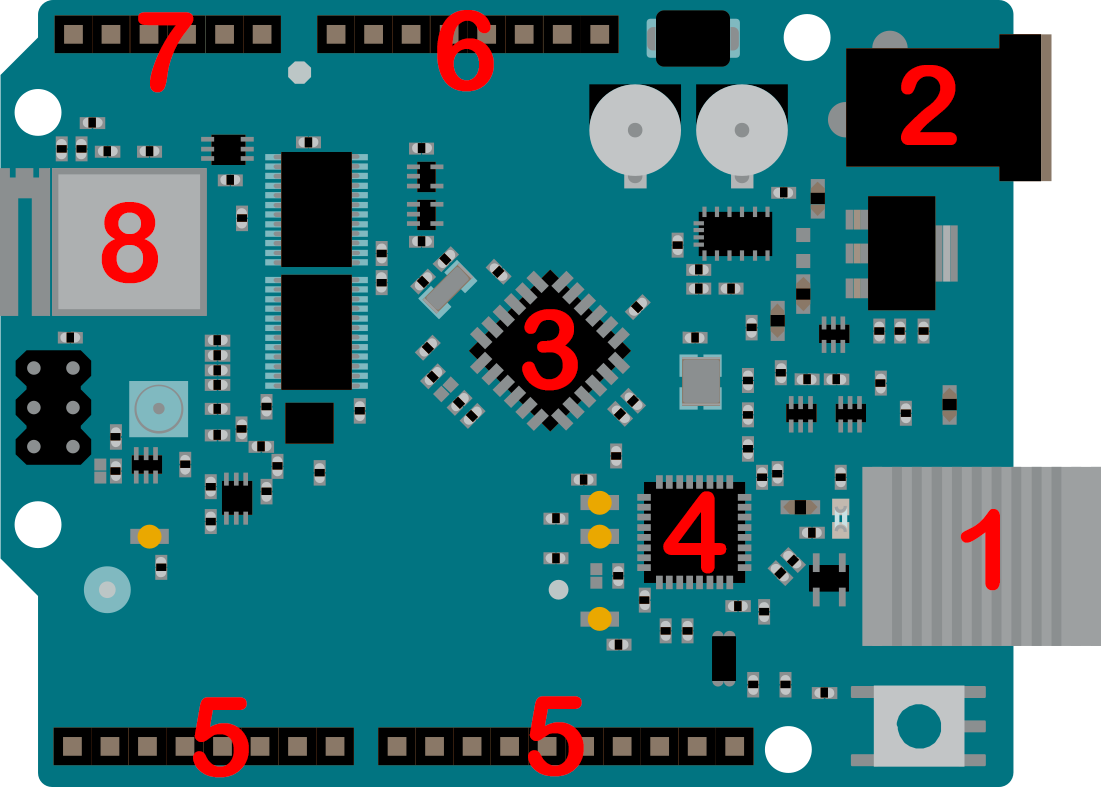
\includegraphics[scale=0.25]{../Quellenangaben/Dokumente/ARDUINO UNO REV2 Dokumentation/unorev2_edited.png}
            \caption[ARDUINOUNOSketch]{Struktur des ARDUINO UNO WIFI REV2 \footnotemark}
            \label{fig:ARDUINOUNOSketch} 
        \end{figure}
            
        \footnotetext{~\citetitle{arduinounorev2doc} \cite{arduinounorev2doc}}

        Das Board besitzt einen Eingang für sogenannte "'Barrel Plugs"' (Abbildung X Markierung Y), welcher der Stromversorgung dient. Er ermöglicht es den ARDUINO mit Spannungen zwischen 6 und 20 Volt zu betreiben. Aufgrund des geringen Strombedarfs des Boards kommen dafür normale Netzgeräte sowie Powerbanks infrage.
        
        Die Stromversorgung kann zusätzlich über einen USB Typ-B Port (Abbildung X Markierung Y) erfolgen. Dieser dient jedoch vor allem zum klassischen Laden von Programmcode über Kabel. 

        Für die USB Verbindung und den ISP Flash besitzt der Arduino einen eigenen Controller (Abbildung X Markierung Y).

        Die zentrale Recheneinheit des Boards ist der Mikroprozessor ATmega4809 (Abbildung X Markierung Y $TODO$), welcher mit Taktraten von 16MHz arbeitet. Er besitzt 48 KB Flash Memory, 6144 Bytes SRAM und einen 256 Bytes großen EEPROM. %TODO Arduino Uno wifi rev2 dokumentation zitieren

        Die Kommunikation mit externer Hardware erfolgt über digitale (Abbildung X Markierung Y) und analoge (Abbildung X Markierung Y) I/O-Pins. Mit diesen können z.B. Werte von Sensoren gelesen oder auch geschrieben werden.
        Die Versorgung der angeschlossenen Hardware erfolgt über separate Power-Pins, die entweder mit 3,3 oder 5 Volt arbeiten.
        
        Die WIFI-Version des Boards besitzt im Vergleich zum Basis-Board zusätzlich ein NINA-W102 WLAN- und Bluetooth-Modul. Über dieses wird die Kommunikation zwischen verschiedenen, räumlich getrennten Geräten und das Hochladen von ARDUINO Sketches "'over the air"' ermöglicht.

        \subsection{Feuchtigkeitssensoren}

        %Verschiedene Messmethoden vorstellen
        Zur Feuchtigkeitsbestimmung mit Hilfe von Sensoren können 2 grundlegende Verfahren verwendet werden. Die einfachste Methode ist dabei die Messung über die elektrische Leitfähigkeit. Hierbei wird mit Hilfe von zwei Elektroden die Leitfähigkeit der zwischen den Elektrodenstäben befindlichen Erde gemessen und von dieser auf die Bodenfeuchte geschlossen. Dieses Verfahren beruht jedoch auf dem direkten Kontakt von Elektroden mit Feuchtigkeit im Boden, wodurch die Elektroden schnell korrodieren. Weiterhin beeinflussen die im Wasser gelösten Salze und Mineralien die Leitfähigkeit wodurch die Messergebnisse unvorhersehbar beeinflusst werden. %TODO DVS Bodenfeuchte zitieren

        Die Alternative zur Messung mit Elektroden ist die kapazitive Messung.
        Hierbei wird ein Kondensator mit einem Dielektrikum verwendet. Das hygroskopische Dielektrikum tauscht dabei Wasserdampf aus dem Boden mit dem Dielektrikum aus. Über eine Messung der Kapazität des Kondensators kann anschließend die relative Feuchte des Bodens über den Wasseranteil des Dielektrikum bestimmt werden. %TODO https://messtechnik-und-sensorik.org/10-sensoren-fuer-temperatur-feuchte-und-gaskonzentrationen/ zitieren
        Dieses Verfahren hat den Vorteil, dass kein direkter Kontakt zwischen dem Boden und den Platten des Kondensators vorliegt und dadurch, bei korrekter Verwendung, praktisch keine Korrosion auftritt.
        Weiterhin kann über dieses Prinzip, eine Auswirkung von im Wasser gelösten Salzen auf das Messergebnis verhindert werden.
        %DVS zitieren

        %Warum haben wir uns für Kapazitive Messung entschieden?
        Auf Grund der Vorteile des kapazitiven Messverfahrens gegenüber dem Messverfahren mit Elektroden wurden im Rahmen dieser Arbeit nur kapazitive Sensoren verwendet.

        %Welche Sensoren haben wir ausgewählt, Spezifikationen?

        Konkret wurde die Sensoren 101020614 von Seeed Studio und SEN0193 von DFRobot verwendet.

        %TODO Abbildung der Sensoren einfügen und referenzieren

        Beide Sensoren lassen sich entweder mit 3,3 oder 5 Volt betreiben und liefern analoge Werte.
        Im direkten Vergleich unterscheiden sich die Messwerte beider Sensoren %TODO Daten vom Test einpflegen 
        
        \subsection{Temperatursensoren}
        \subsection{Lichtsensor}
        \subsection{Arduino IDE}
    \section{Konzept}
        \subsection{Zusammenhang Module}
        \subsection{Messmodul}
        \subsection{Speichermodul}
        \subsection{Auswertungsmodul}
        \subsection{Automatisierungsmodul}
    \section{Implementierung}
        \subsection{Zusammenhang Module}
        \subsection{Messmodul}
        \subsection{Speichermodul}
        \subsection{Auswertungsmodul}
        \subsection{Automatisierungsmodul}
    
\chapter{Ergebnis}
    (Kopie der Aufgabenstellung mit gelöst/gelöst, vielleicht als Tabelle)
    
\chapter{Kritische Reflexion}
    (Stellung nehmen zum Ergebnis)
    (Eigene Meinung zum Ergebnis)

\chapter{Ausblick}
    (Erweiterungsmöglichkeiten)
    (Coole weitere Funktionen)
    (Was kann verbessert werden?)

%gibt das literaturverzeichnis aus    
%\printbibliography
%Anhang    
\appendix
\chapter{Begriffsdefinitionen}

\section{Begriffsbezeichner} \label{sec:Begriffsbezeichner}




\chapter{Abkürzungsverzeichnis}


%Deklaration von Acronymen    
\begin{acronym}[nonumberlist]

%\acro{Bezeichner}[Abkürzung im Text]{Ausgeschriebene Bezeichnung}
%Bsp:
%\acro{dlr}[DLR]{Deutsches Zentrum für Luft- und Raumfahrt}


\end{acronym} 

\nocite{*}

\end{document}